\documentclass[twoside]{book}

% Packages required by doxygen
\usepackage{calc}
\usepackage{doxygen}
\usepackage{graphicx}
\usepackage[utf8]{inputenc}
\usepackage{makeidx}
\usepackage{multicol}
\usepackage{multirow}
\usepackage{textcomp}
\usepackage[table]{xcolor}

% Font selection
\usepackage[T1]{fontenc}
\usepackage{mathptmx}
\usepackage[scaled=.90]{helvet}
\usepackage{courier}
\usepackage{amssymb}
\usepackage{sectsty}
\renewcommand{\familydefault}{\sfdefault}
\allsectionsfont{%
  \fontseries{bc}\selectfont%
  \color{darkgray}%
}
\renewcommand{\DoxyLabelFont}{%
  \fontseries{bc}\selectfont%
  \color{darkgray}%
}

% Page & text layout
\usepackage{geometry}
\geometry{%
  a4paper,%
  top=2.5cm,%
  bottom=2.5cm,%
  left=2.5cm,%
  right=2.5cm%
}
\tolerance=750
\hfuzz=15pt
\hbadness=750
\setlength{\emergencystretch}{15pt}
\setlength{\parindent}{0cm}
\setlength{\parskip}{0.2cm}
\makeatletter
\renewcommand{\paragraph}{%
  \@startsection{paragraph}{4}{0ex}{-1.0ex}{1.0ex}{%
    \normalfont\normalsize\bfseries\SS@parafont%
  }%
}
\renewcommand{\subparagraph}{%
  \@startsection{subparagraph}{5}{0ex}{-1.0ex}{1.0ex}{%
    \normalfont\normalsize\bfseries\SS@subparafont%
  }%
}
\makeatother

% Headers & footers
\usepackage{fancyhdr}
\pagestyle{fancyplain}
\fancyhead[LE]{\fancyplain{}{\bfseries\thepage}}
\fancyhead[CE]{\fancyplain{}{}}
\fancyhead[RE]{\fancyplain{}{\bfseries\leftmark}}
\fancyhead[LO]{\fancyplain{}{\bfseries\rightmark}}
\fancyhead[CO]{\fancyplain{}{}}
\fancyhead[RO]{\fancyplain{}{\bfseries\thepage}}
\fancyfoot[LE]{\fancyplain{}{}}
\fancyfoot[CE]{\fancyplain{}{}}
\fancyfoot[RE]{\fancyplain{}{\bfseries\scriptsize Generated on Mon Mar 24 2014 15\-:18\-:36 for Sound\-Recorder by Doxygen }}
\fancyfoot[LO]{\fancyplain{}{\bfseries\scriptsize Generated on Mon Mar 24 2014 15\-:18\-:36 for Sound\-Recorder by Doxygen }}
\fancyfoot[CO]{\fancyplain{}{}}
\fancyfoot[RO]{\fancyplain{}{}}
\renewcommand{\footrulewidth}{0.4pt}
\renewcommand{\chaptermark}[1]{%
  \markboth{#1}{}%
}
\renewcommand{\sectionmark}[1]{%
  \markright{\thesection\ #1}%
}

% Indices & bibliography
\usepackage{natbib}
\usepackage[titles]{tocloft}
\setcounter{tocdepth}{3}
\setcounter{secnumdepth}{5}
\makeindex

% Hyperlinks (required, but should be loaded last)
\usepackage{ifpdf}
\ifpdf
  \usepackage[pdftex,pagebackref=true]{hyperref}
\else
  \usepackage[ps2pdf,pagebackref=true]{hyperref}
\fi
\hypersetup{%
  colorlinks=true,%
  linkcolor=blue,%
  citecolor=blue,%
  unicode%
}

% Custom commands
\newcommand{\clearemptydoublepage}{%
  \newpage{\pagestyle{empty}\cleardoublepage}%
}


%===== C O N T E N T S =====

\begin{document}

% Titlepage & ToC
\hypersetup{pageanchor=false}
\pagenumbering{roman}
\begin{titlepage}
\vspace*{7cm}
\begin{center}%
{\Large Sound\-Recorder \\[1ex]\large 1.\-0.\-0 }\\
\vspace*{1cm}
{\large Generated by Doxygen 1.8.6}\\
\vspace*{0.5cm}
{\small Mon Mar 24 2014 15:18:36}\\
\end{center}
\end{titlepage}
\clearemptydoublepage
\tableofcontents
\clearemptydoublepage
\pagenumbering{arabic}
\hypersetup{pageanchor=true}

%--- Begin generated contents ---
\chapter{Bug List}
\label{bug}
\hypertarget{bug}{}

\begin{DoxyRefList}
\item[\label{bug__bug000001}%
\hypertarget{bug__bug000001}{}%
File \hyperlink{main_8cpp}{main.cpp} ]No known bugs. 
\end{DoxyRefList}
\chapter{Hierarchical Index}
\section{Class Hierarchy}
This inheritance list is sorted roughly, but not completely, alphabetically\-:\begin{DoxyCompactList}
\item $<$A\-V\-Audio\-Player\-Delegate$>$\begin{DoxyCompactList}
\item \contentsline{section}{S\-E\-Sound()}{\pageref{category_s_e_sound_07_08}}{}
\end{DoxyCompactList}
\item $<$A\-V\-Audio\-Recorder\-Delegate$>$\begin{DoxyCompactList}
\item \contentsline{section}{S\-E\-Sound()}{\pageref{category_s_e_sound_07_08}}{}
\end{DoxyCompactList}
\item N\-S\-Object\begin{DoxyCompactList}
\item \contentsline{section}{S\-E\-Audio\-Stream}{\pageref{interface_s_e_audio_stream}}{}
\item \contentsline{section}{S\-E\-Audio\-Stream\-Player}{\pageref{interface_s_e_audio_stream_player}}{}
\item \contentsline{section}{S\-E\-Sound}{\pageref{interface_s_e_sound}}{}
\item \contentsline{section}{S\-R\-Audio\-Stream\-Player}{\pageref{interface_s_r_audio_stream_player}}{}
\end{DoxyCompactList}
\item $<$N\-S\-Object\-N\-S\-Object$>$\begin{DoxyCompactList}
\item \contentsline{section}{$<$S\-E\-Audio\-Stream\-Player\-Delegate$>$}{\pageref{protocol_s_e_audio_stream_player_delegate-p}}{}
\item \contentsline{section}{$<$S\-R\-Audio\-Stream\-Delegate$>$}{\pageref{protocol_s_r_audio_stream_delegate-p}}{}
\item \contentsline{section}{$<$S\-R\-Sound\-Delegate$>$}{\pageref{protocol_s_r_sound_delegate-p}}{}
\end{DoxyCompactList}
\item \contentsline{section}{S\-E\-Audio\-Stream(Read)}{\pageref{category_s_e_audio_stream_07_read_08}}{}
\item \contentsline{section}{S\-E\-Audio\-Stream(Write)}{\pageref{category_s_e_audio_stream_07_write_08}}{}
\item \contentsline{section}{S\-E\-Project()}{\pageref{category_s_e_project_07_08}}{}
\item \contentsline{section}{S\-R\-Audio\-Stream\-Player()}{\pageref{category_s_r_audio_stream_player_07_08}}{}
\item S\-R\-Model\begin{DoxyCompactList}
\item \contentsline{section}{S\-E\-Project}{\pageref{interface_s_e_project}}{}
\item \contentsline{section}{S\-E\-Record}{\pageref{interface_s_e_record}}{}
\end{DoxyCompactList}
\item \contentsline{section}{S\-R\-Sound\-Range}{\pageref{struct_s_r_sound_range}}{}
\end{DoxyCompactList}

\chapter{Class Index}
\section{Class List}
Here are the classes, structs, unions and interfaces with brief descriptions\-:\begin{DoxyCompactList}
\item\contentsline{section}{\hyperlink{class_application_u_i}{Application\-U\-I} \\*Application object }{\pageref{class_application_u_i}}{}
\end{DoxyCompactList}

\chapter{File Index}
\section{File List}
Here is a list of all files with brief descriptions\-:\begin{DoxyCompactList}
\item\contentsline{section}{Sound\-Recorder/\-Classes/\-Core/\-Sound\-Editor/\hyperlink{_s_e_audio_stream_8h}{S\-E\-Audio\-Stream.\-h} }{\pageref{_s_e_audio_stream_8h}}{}
\item\contentsline{section}{Sound\-Recorder/\-Classes/\-Core/\-Sound\-Editor/\hyperlink{_s_e_audio_stream_8m}{S\-E\-Audio\-Stream.\-m} }{\pageref{_s_e_audio_stream_8m}}{}
\item\contentsline{section}{Sound\-Recorder/\-Classes/\-Core/\-Sound\-Editor/\hyperlink{_s_e_audio_stream_player_8h}{S\-E\-Audio\-Stream\-Player.\-h} }{\pageref{_s_e_audio_stream_player_8h}}{}
\item\contentsline{section}{Sound\-Recorder/\-Classes/\-Core/\-Sound\-Editor/\hyperlink{_s_e_audio_stream_player_8m}{S\-E\-Audio\-Stream\-Player.\-m} }{\pageref{_s_e_audio_stream_player_8m}}{}
\item\contentsline{section}{Sound\-Recorder/\-Classes/\-Core/\-Sound\-Editor/\hyperlink{_s_e_project_8h}{S\-E\-Project.\-h} }{\pageref{_s_e_project_8h}}{}
\item\contentsline{section}{Sound\-Recorder/\-Classes/\-Core/\-Sound\-Editor/\hyperlink{_s_e_project_8mm}{S\-E\-Project.\-mm} }{\pageref{_s_e_project_8mm}}{}
\item\contentsline{section}{Sound\-Recorder/\-Classes/\-Core/\-Sound\-Editor/\hyperlink{_s_e_record_8h}{S\-E\-Record.\-h} }{\pageref{_s_e_record_8h}}{}
\item\contentsline{section}{Sound\-Recorder/\-Classes/\-Core/\-Sound\-Editor/\hyperlink{_s_e_record_8m}{S\-E\-Record.\-m} }{\pageref{_s_e_record_8m}}{}
\item\contentsline{section}{Sound\-Recorder/\-Classes/\-Core/\-Sound\-Editor/\hyperlink{_s_e_sound_8h}{S\-E\-Sound.\-h} }{\pageref{_s_e_sound_8h}}{}
\item\contentsline{section}{Sound\-Recorder/\-Classes/\-Core/\-Sound\-Editor/\hyperlink{_s_e_sound_8m}{S\-E\-Sound.\-m} }{\pageref{_s_e_sound_8m}}{}
\item\contentsline{section}{Sound\-Recorder/\-Classes/\-Core/\-Sound\-Editor/\hyperlink{_s_r_audio_stream_player_8h}{S\-R\-Audio\-Stream\-Player.\-h} }{\pageref{_s_r_audio_stream_player_8h}}{}
\item\contentsline{section}{Sound\-Recorder/\-Classes/\-Core/\-Sound\-Editor/\hyperlink{_s_r_audio_stream_player_8m}{S\-R\-Audio\-Stream\-Player.\-m} }{\pageref{_s_r_audio_stream_player_8m}}{}
\end{DoxyCompactList}

\chapter{Class Documentation}
\hypertarget{class_application_u_i}{\section{Application\-U\-I Class Reference}
\label{class_application_u_i}\index{Application\-U\-I@{Application\-U\-I}}
}


Application object.  




{\ttfamily \#include $<$applicationui.\-hpp$>$}

Inheritance diagram for Application\-U\-I\-:\begin{figure}[H]
\begin{center}
\leavevmode
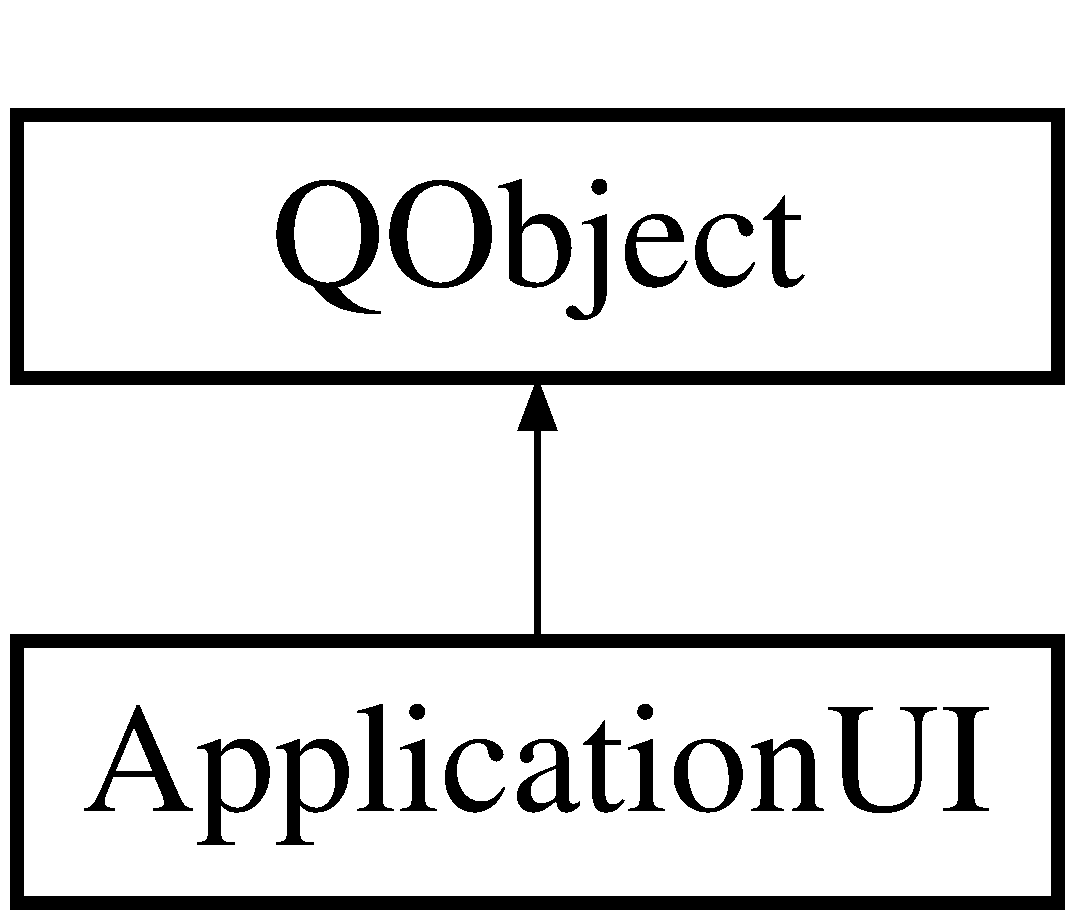
\includegraphics[height=2.000000cm]{class_application_u_i}
\end{center}
\end{figure}
\subsection*{Public Member Functions}
\begin{DoxyCompactItemize}
\item 
\hypertarget{class_application_u_i_a1799d0645a3a41aec6bec5379e875d0a}{{\bfseries Application\-U\-I} (bb\-::cascades\-::\-Application $\ast$app)}\label{class_application_u_i_a1799d0645a3a41aec6bec5379e875d0a}

\end{DoxyCompactItemize}


\subsection{Detailed Description}
Application object. 

The documentation for this class was generated from the following files\-:\begin{DoxyCompactItemize}
\item 
src/applicationui.\-hpp\item 
src/applicationui.\-cpp\end{DoxyCompactItemize}

\chapter{File Documentation}
\hypertarget{main_8cpp}{\section{src/main.cpp File Reference}
\label{main_8cpp}\index{src/main.\-cpp@{src/main.\-cpp}}
}


d-\/dimensional point class  


{\ttfamily \#include $<$bb/cascades/\-Application$>$}\\*
{\ttfamily \#include $<$Q\-Locale$>$}\\*
{\ttfamily \#include $<$Q\-Translator$>$}\\*
{\ttfamily \#include \char`\"{}applicationui.\-hpp\char`\"{}}\\*
{\ttfamily \#include $<$Qt/qdeclarativedebug.\-h$>$}\\*
\subsection*{Functions}
\begin{DoxyCompactItemize}
\item 
\hypertarget{main_8cpp_ac524bcebfc171d953d2944b13b2d0eb4}{Q\-\_\-\-D\-E\-C\-L\-\_\-\-E\-X\-P\-O\-R\-T int {\bfseries main} (int argc, char $\ast$$\ast$argv)}\label{main_8cpp_ac524bcebfc171d953d2944b13b2d0eb4}

\end{DoxyCompactItemize}


\subsection{Detailed Description}
d-\/dimensional point class \begin{DoxyAuthor}{Author}
Timofey Kovalenko (\href{mailto:timothy.kovalenko@wise-apps.com}{\tt timothy.\-kovalenko@wise-\/apps.\-com}) 
\end{DoxyAuthor}
\begin{DoxyRefDesc}{Bug}
\item[\hyperlink{bug__bug000001}{Bug}]No known bugs. \end{DoxyRefDesc}

%--- End generated contents ---

% Index
\newpage
\phantomsection
\addcontentsline{toc}{chapter}{Index}
\printindex

\end{document}
